\chapter{Resultados} \label{cap:resultados}

Este capítulo apresenta os resultados obtidos e discute as implicações do estudo comparativo. Os resultados são apresentados em tabelas e gráficos, seguidos de uma análise detalhada do que fora observado.

\section{Métricas Gerais de Desempenho}

Os resultados das métricas de desempenho geral dos modelos de RNC e ViT são apresentados na \autoref{tab:overall_metrics_all_models}. A acurácia geral variou de 0.6894 (DeiT-Distilled-B) a 0.7885 (DenseNet-169), com o modelo DenseNet-169 alcançando a maior acurácia com uso da entropia cruzada. No entanto, considerando a característica ordinal da classificação, a métrica QWK oferece uma visão mais precisa do desempenho dos modelos. O modelo DenseNet-121 obteve o melhor QWK de 0.8878, seguido pelo GCViT-B com QWK de 0.8832, ambos com uso da entropia cruzada. No geral, esses resultados sugerem que os modelos da família DenseNet foram particularmente úteis para capturar as características visuais da OA de joelho, principalmente devido à sua arquitetura densa que permite que as camadas mais profundas acessem diretamente as características de baixo nível, sem precisar reaprendê-las \citep{Huang2017}.

\begin{table}[ht]
    \centering
    \begin{tabular}{llccc}
        \toprule
        \textbf{Modelo} & \textbf{Função de perda} & \textbf{Acurácia} & \textbf{QWK} & \textbf{MAE} \\
        \midrule
        ResNet-34 & \text{Entropia cruzada} & 0.7258 & 0.8475 & 0.3282 \\
        ResNet-34 & \text{CORN} & 0.7203 & 0.8568 & 0.3194 \\
        ResNet-50 & \text{Entropia cruzada} & 0.7478 & 0.8509 & 0.3095 \\
        ResNet-50 & \text{CORN} & 0.7379 & 0.8779 & 0.2874 \\
        ResNet-101 & \text{Entropia cruzada} & 0.7445 & 0.8556 & 0.3040 \\
        ResNet-101 & \text{CORN} & 0.7214 & 0.8633 & 0.3128 \\
        VGG-16 & \text{Entropia cruzada} & 0.7159 & 0.8534 & 0.3293 \\
        VGG-16 & \text{CORN} & 0.7115 & 0.8614 & 0.3216 \\
        VGG-19 & \text{Entropia cruzada} & 0.7048 & 0.8522 & 0.3370 \\
        VGG-19 & \text{CORN} & 0.7037 & 0.8596 & 0.3260 \\
        DenseNet-121 & \text{Entropia cruzada} & 0.7709 & \textbf{0.8878} & 0.2599 \\
        DenseNet-121 & \text{CORN} & 0.7357 & 0.8830 & 0.2852 \\
        DenseNet-169 & \text{Entropia cruzada} & \textbf{0.7885} & 0.8811 & \textbf{0.2522} \\
        DenseNet-169 & \text{CORN} & 0.7324 & 0.8767 & 0.2919 \\
        Inception-v3 & \text{Entropia cruzada} & 0.7247 & 0.8571 & 0.3172 \\
        Inception-v3 & \text{CORN} & 0.7533 & 0.8813 & 0.2742 \\
        DeiT-Distilled-B & \text{Entropia cruzada} & 0.6938 & 0.8321 & 0.3634 \\
        DeiT-Distilled-B & \text{CORN} & 0.6960 & 0.8514 & 0.3381 \\
        DaViT-B & \text{Entropia cruzada} & 0.7709 & 0.8758 & 0.2687 \\
        DaViT-B & \text{CORN} & 0.7357 & 0.8700 & 0.2974 \\
        MaxViT-T & \text{Entropia cruzada} & 0.7467 & 0.8778 & 0.2841 \\
        MaxViT-T & \text{CORN} & 0.7456 & 0.8800 & 0.2819 \\
        GCViT-B & \text{Entropia cruzada} & 0.7555 & 0.8832 & 0.2742 \\
        GCViT-B & \text{CORN} & 0.7335 & 0.8804 & 0.2896 \\
        Swin-B & \text{Entropia cruzada} & 0.7059 & 0.8463 & 0.3425 \\
        Swin-B & \text{CORN} & 0.7026 & 0.8617 & 0.3293 \\
        \bottomrule
    \end{tabular}
    \caption{Métricas de desempenho de cada modelo na tarefa de classificar a OA de joelho em cinco classes, considerando as funções de perda Entropia Cruzada e CORN.}
    \label{tab:overall_metrics_all_models}
\end{table}

A avaliação comparativa das funções de perda revelou um claro \textit{trade-off} entre a acurácia categórica e a correção ordinal. Na maioria dos cenários, os modelos treinados com a função de perda de entropia cruzada apresentaram um desempenho superior em termos de acurácia, com uma média de 1,58\% a mais em relação aos seus equivalentes treinados com a função CORN. Isso sugere que a entropia cruzada é mais eficaz para maximizar o número de classificações exatamente corretas.

Em contrapartida, a função CORN demonstrou sua superioridade em métricas que avaliam a natureza ordinal do problema. Observou-se um aumento médio de 1,06\% no QWK, como exemplificado pelo modelo Inception-v3, cujo QWK aumentou de 0.8571 para 0.8813. Adicionalmente, houve uma redução de 0,89\% no Erro Absoluto Médio (MAE), confirmando a eficácia do CORN em minimizar a magnitude dos erros de predição.

Portanto, a escolha da função de perda está muito ligada ao objetivo da aplicação. Para maximizar a precisão categórica, a entropia cruzada é a abordagem preferível. No entanto, em um contexto de suporte à decisão clínica, onde um erro ordinal pequeno (por exemplo, prever KL-2 para um KL-3 real) é significativamente menos crítico do que um erro grande (por exemplo, prever KL-0), a função CORN é mais adequada. Isso se deve à sua capacidade de gerar modelos que, mesmo quando erram, produzem predições mais próximas do rótulo verdadeiro, alinhando-se melhor à relevância clínica dos erros.

% A \autoref{tab:resultados} mostra a acurácia dos modelos de RNCs e ViTs treinados para a classificação da OA de joelho usando a função de perda \textit{crossentropy}. Em relação ao tempo de treinamento, é possível notar que o modelo mais rápido foi o ResNet-50, com um tempo de 11.29 segundos. Por outro lado, o modelo mais lento foi o DeiT, com um tempo de 79.5 segundos. Tais valores não necessariamente indicam que o modelo mais rápido é o pior, ou o contrário, mas é importante considerar o tempo de treinamento como um fator relevante ao escolher um modelo, especialmente se houver restrições de recursos computacionais. O tempo de treinamento mostrado varia, principalmente, com o número de épocas, já que modelos que levaram mais tempo são aqueles que tiveram a parada antecipada mais tarde, ou executaram as 30 épocas completas.

\section{Métricas de Desempenho por Classe}

A análise detalhada dos F1-scores por classe, apresentada na \autoref{tab:f1_scores_all_models}, revela padrões de desempenho que vão além da simples identificação de um modelo superior. Os resultados expõem a complexidade intrínseca da classificação da escala KL e destacam como diferentes arquiteturas respondem a cada estágio da doença.

A tabela revela a observação central onde o desempenho dos modelos é consistentemente baixo na classe KL-1 (duvidoso). Nenhum modelo, independentemente da arquitetura (RNC ou ViT) ou da função de perda, consegui superar um F1-score de 0.60 para esta classe, com o melhor sendo o DenseNet-169 (0.5970) e o pior sendo o VGG-19 (0.3750). Esse resultado sugere que a classe KL-1 é inerentemente ambígua e inconsistente, assim como diz \cite{Spector1993}. Ela representa um estágio da OA, onde os achados radiológicos, como um possível estreitamento do espaço articular ou a formação de osteófitos, são muito sutis. Como consequência, essa classe sofre com a sobreposição de características entre as classes adjacentes, tornando a classificação pelos modelos mais desafiadora.

Em forte contraste com a classe KL-1, as classes nos extremos da escala, KL-0 (saudável) e KL-4 (severo), apresentam F1-scores consistentemente altos na maioria dos modelos. Para a classe KL-0, modelos como DenseNet-121 (0.8454) e GCViT-B (0.8409) demostraram uma boa capacidade de identificar corretamente um joelho saudável. Já para a classe KL-4, os resultados são ainda mais expressivos, com modelos como DaViT-B e MaxViT-T alcançando F1-scores muito elevados (ambos com 0.9310).

As classes KL-2 (mínimo) e KL-3 (moderado) representam estágios onde a doença já está presente e o desempenho dos modelos foi mais equilibrado. Modelos como DaViT-B (0.9212 para KL-3) e DenseNet-169 (0.9016 para KL-3) mostraram uma capacidade notável de distinguir os estágios intermediários da doença.

Essa análise por classe não apenas valida a decisão de realizar experimentos excluindo a classe KL-1, mas também confirma que o desempenho dos modelos está fortemente alinhado à realidade clínica da OA de joelho: alta certeza nos casos extremos e dificuldade na zona de transição (KL-1).

\begin{sidewaystable}[ht]
    \centering
    \begin{tabular}{llcccccc}
        \toprule
        \textbf{Modelo} & \textbf{Função de perda} & \textbf{Média Macro} & \textbf{KL-0} & \textbf{KL-1} & \textbf{KL-2} & \textbf{KL-3} & \textbf{KL-4} \\
        \midrule
        ResNet-34 & \text{Entropia cruzada} & 0.7384 & 0.7932 & 0.4669 & 0.7187 & 0.8465 & 0.8667 \\
        ResNet-34 & \text{CORN} & 0.7431 & 0.8034 & 0.5117 & 0.6837 & 0.8354 & 0.8814 \\
        ResNet-50 & \text{Entropia cruzada} & 0.7722 & 0.7983 & 0.5257 & 0.7364 & 0.8852 & 0.9153 \\
        ResNet-50 & \text{CORN} & 0.7564 & 0.8239 & 0.5158 & 0.7244 & 0.8326 & 0.8852 \\
        ResNet-101 & \text{Entropia cruzada} & 0.7726 & 0.7983 & 0.5683 & 0.7277 & 0.8534 & 0.9153 \\
        ResNet-101 & \text{CORN} & 0.7359 & 0.8142 & 0.4932 & 0.6920 & 0.8412 & 0.8387 \\
        VGG-16 & \text{Entropia cruzada} & 0.7276 & 0.8063 & 0.4201 & 0.6912 & 0.8537 & 0.8667 \\
        VGG-16 & \text{CORN} & 0.7384 & 0.7935 & 0.4358 & 0.7042 & 0.8583 & 0.9000 \\
        VGG-19 & \text{Entropia cruzada} & 0.7066 & 0.7898 & 0.3750 & 0.7146 & 0.8468 & 0.8070 \\
        VGG-19 & \text{CORN} & 0.7268 & 0.7935 & 0.4216 & 0.6949 & 0.8667 & 0.8571 \\
        DenseNet-121 & \text{Entropia cruzada} & 0.7777 & 0.8454 & 0.5378 & 0.7537 & 0.8807 & 0.8710 \\
        DenseNet-121 & \text{CORN} & 0.7563 & 0.8192 & 0.4890 & 0.7292 & 0.8439 & 0.9000 \\
        DenseNet-169 & \text{Entropia cruzada} & 0.8061 & 0.8384 & 0.5970 & 0.7780 & 0.9016 & 0.9153 \\
        DenseNet-169 & \text{CORN} & 0.7583 & 0.8066 & 0.5433 & 0.7097 & 0.8608 & 0.8710 \\
        Inception-v3 & \text{Entropia cruzada} & 0.7487 & 0.7959 & 0.4734 & 0.7166 & 0.8455 & 0.9123 \\
        Inception-v3 & \text{CORN} & 0.7811 & 0.8067 & 0.5464 & 0.7589 & 0.8780 & 0.9153 \\
        DeiT-Distilled-B & \text{Entropia cruzada} & 0.7206 & 0.7670 & 0.3938 & 0.6790 & 0.8631 & 0.9000 \\
        DeiT-Distilled-B & \text{CORN} & 0.7378 & 0.7527 & 0.4230 & 0.7157 & 0.8852 & 0.9123 \\
        DaViT-B & \text{Entropia cruzada} & 0.7968 & 0.8111 & 0.5401 & 0.7807 & 0.9212 & 0.9310 \\
        DaViT-B & \text{CORN} & 0.7622 & 0.7912 & 0.4756 & 0.7510 & 0.8807 & 0.9123 \\
        MaxViT-T & \text{Entropia cruzada} & 0.7649 & 0.8329 & 0.4986 & 0.7143 & 0.8787 & 0.9000 \\
        MaxViT-T & \text{CORN} & 0.7728 & 0.8333 & 0.4945 & 0.7100 & 0.8952 & 0.9310 \\
        GCViT-B & \text{Entropia cruzada} & 0.7720 & 0.8409 & 0.5128 & 0.7136 & 0.8926 & 0.9000 \\
        GCViT-B & \text{CORN} & 0.7459 & 0.8093 & 0.4501 & 0.7463 & 0.8760 & 0.8475 \\
        Swin-B & \text{Entropia cruzada} & 0.7237 & 0.7944 & 0.4037 & 0.6795 & 0.8595 & 0.8814 \\
        Swin-B & \text{CORN} & 0.7261 & 0.7994 & 0.4261 & 0.6681 & 0.8405 & 0.8966 \\
        \bottomrule
    \end{tabular}
    \caption{Métrica F1-score para cada uma das cinco classes e modelo, considerando as funções de perda Entropia Cruzada e CORN.}
    \label{tab:f1_scores_all_models}
\end{sidewaystable}

\section{Eficiência Computacional}

A análise dos tempos de treinamento e inferência, apresentada na \autoref{tab:computational_performance}, revela distinções cruciais entre os modelos e funções de perda, oferecendo um respaldo da aplicação prática e que complementa as métricas de desempenho preditivo.

O tempo de inferência por imagem é uma métrica crítica para a aplicação clínica, e as RNCs demonstram uma vantagem sobre os ViTs. Modelos como ResNet-34 (1,55 ms/imagem), ResNet-50 (2,87 ms/imagem) e DenseNet/121 (3,11 ms/imagem) são os mais rápidos, estabelecendo uma linha de base de alta eficiência. Suas arquiteturas são bem otimizadas para o hardware de GPU, o que permite um processamento rápido.

Em contraste, os ViTs apresentaram tempos de inferência significativamente mais altos. O mais rápido entre eles, MaxViT-T (6,92 ms/imagem), já é mais de duas vezes mais lento do que as RNCs eficientes. Essa disparidade pode ser justificada pela natureza das operações. Embora ViTs tenham alcançado complexidade computacional linear em relação ao tamanho de imagem, como citam \cite{ding2022davitdualattentionvision} e \cite{maxvit2022}, seus blocos de atenção ainda envolvem operações de multiplicação de matrizes em larga escala que são mais custosas do que as operações de convolução. Isso também pode ser visualizado na \autoref{tab:model_list}, na coluna de FLOPs (GMac).

A literatura sobre modelos como MaxViT e DaViT foca em tornar a atenção global mais eficiente e de fato tornam, mas os resultados práticos da \autoref{tab:computational_performance} demonstram que, na GPU utilizada, a sobrecarga computacional da auto-atenção ainda é um obstáculo significativo para a inferência quando comparada às RNCs.

% Ao observar o custo computacional pela \autoref{tab:computational_performance}, nota-se que esses modelos de ViT são mais pesados em termos de FLOPs (15.28 GMac e 13.89 GMac) e parâmetros (86.93 M e 89.3 M), o que impacta no tempo de treinamento. Nesse sentido, arquiteturas da família DenseNet demonstram ser mais eficientes, com o DenseNet-169 usando apenas 12.49 M de parâmetros e 3.44 GMac FLOPs, ou seja, seis quatro menos parâmetros FLOPs do que o DaViT-B (CE).

\begin{sidewaystable}[ht]
    \centering
    \begin{tabular}{llccc}
        \toprule
        \textbf{Modelo} & \textbf{Função de perda} & \textbf{Treinamento (min)} & \textbf{Inferência média/batch (ms)} & \textbf{Inferência média/imagem (ms)} \\
        \midrule
        ResNet-34 & Entropia Cruzada & 33.46 & 43.53 & 1.55 \\
        ResNet-34 & CORN & 89.29 & 43.71 & 1.56 \\
        ResNet-50 & Entropia Cruzada & 14.55 & 80.45 & 2.87 \\
        ResNet-50 & CORN & 9.87 & 80.83 & 2.89 \\
        ResNet-101 & Entropia Cruzada & 22.02 & 137.90 & 4.93 \\
        ResNet-101 & CORN & 16.94 & 139.76 & 4.99 \\
        VGG-16 & Entropia Cruzada & 37.70 & 128.08 & 4.57 \\
        VGG-16 & CORN & 28.45 & 126.44 & 4.52 \\
        VGG-19 & Entropia Cruzada & 39.32 & 153.06 & 5.47 \\
        VGG-19 & CORN & 34.68 & 154.96 & 5.53 \\
        DenseNet-121 & Entropia Cruzada & 12.74 & 87.02 & 3.11 \\
        DenseNet-121 & CORN & 9.22 & 87.26 & 3.12 \\
        DenseNet-169 & Entropia Cruzada & 15.06 & 108.95 & 3.89 \\
        DenseNet-169 & CORN & 16.72 & 108.48 & 3.87 \\
        Inception-v3 & Entropia Cruzada & 12.52 & 108.58 & 3.88 \\
        Inception-v3 & CORN & 14.39 & 108.86 & 3.89 \\
        DeiT-Distilled-B & Entropia Cruzada & 77.31 & 331.55 & 11.84 \\
        DeiT-Distilled-B & CORN & 40.20 & 330.48 & 11.80 \\
        DaViT-B & Entropia Cruzada & 57.83 & 335.72 & 11.99 \\
        DaViT-B & CORN & 27.08 & 339.09 & 12.11 \\
        MaxViT-T & Entropia Cruzada & 28.03 & 193.82 & 6.92 \\
        MaxViT-T & CORN & 29.36 & 194.79 & 6.96 \\
        GCViT-B & Entropia Cruzada & 49.57 & 408.07 & 14.57 \\
        GCViT-B & CORN & 34.65 & 409.04 & 14.61 \\
        Swin-B & Entropia Cruzada & 46.61 & 344.37 & 12.30 \\
        Swin-B & CORN & 36.02 & 348.65 & 12.45 \\
        \bottomrule
    \end{tabular}
    \caption{Tempos de treinamento e inferência de cada modelo.}
    \label{tab:computational_performance}
\end{sidewaystable}

% \section{RNCs e ViTs}

\section{Análise Quantitativa}

A predição conformal foi aplicada para quantificar a incerteza dos modelos, gerando conjuntos de predição com um nível de confiança estatisticamente garantido de 95\%. A análise dos resultados da \autoref{tab:conformal_coverage} sugere um \textit{trade-off} entre a robustez da garantia de cobertura e a utilidade prática dos conjuntos de predição.

Como descrito na \autoref{sec:conformal-prediction}, a cobertura mede a porcentagem de vezes que a classe verdadeira esteve contida no conjunto de predição conformal no conjunto de teste. Modelos com entropia cruzada demonstraram uma cobertura muito alta, consistentemente alcançando valores de 100\%, como é o caso do ResNet-50, VGG-16, DenseNet-121, DeiT-Distilled e Swin-B. Embora isso satisfaça a garantia teórica de cobrir pelo menos 95\% dos casos, valores altos sugerem que o método é excessivamente conservador, com valores de $\hat{q}$ muito alto.

Já a cobertura para os modelos com CORN for mais variável, geralmente situando-se mais próxima ao objetivo de 95\%, exemplo do ResNet-50 (93,61\%) e Inception-v3 (94,16\%). No entanto, alguns modelos apresentaram uma cobertura abaixo do esperado, como o DenseNet-121, com 86,67\%, indicando que a abordagem ordinal, embora mais ``justa'' em sua calibração, pode ser menos estável em garantir a cobertura em todos os casos.

A utilidade do método de predição conformal é inversamente proporcional ao tamanho dos conjuntos de predição gerados, ou seja, conjuntos menores indicam maior confiança e são mais informativos. Nesse sentido, a abordagem ordinal com CORN desmonstrou uma superioridade.

% TODO: adicionar analise com base no tamanho dos sets

\begin{table}[ht]
    \centering
    \begin{tabular}{llr}
        \toprule
        \textbf{Modelo} & \textbf{Função de perda} & \textbf{Cobertura} \\
        \midrule
            ResNet-34 & Entropia Cruzada &    0.9989 \\
            ResNet-34 & CORN &    0.8822 \\
            ResNet-50 & Entropia Cruzada &    1.0000 \\
            ResNet-50 & CORN &    0.9361 \\
            ResNet-101 & Entropia Cruzada &    0.9956 \\
            ResNet-101 & CORN &    0.8844 \\
            VGG-16 & Entropia Cruzada &    1.0000 \\
            VGG-16 & CORN &    0.9273 \\
            VGG-19 & Entropia Cruzada &    0.9989 \\
            VGG-19 & CORN &    0.9262 \\
            DenseNet-121 & Entropia Cruzada &    1.0000 \\
            DenseNet-121 & CORN &    0.8667 \\
            DenseNet-169 & Entropia Cruzada &    0.9989 \\
            DenseNet-169 & CORN &    0.9163 \\
            Inception-v3 & Entropia Cruzada &    0.9989 \\
            Inception-v3 & CORN &    0.9416 \\
            DeiT-Distilled-B & Entropia Cruzada &    1.0000 \\
            DeiT-Distilled-B & CORN &    0.9163 \\
            DaViT-B & Entropia Cruzada &    0.9989 \\
            DaViT-B & CORN &    0.8844 \\
            MaxViT-T & Entropia Cruzada &    0.9989 \\
            MaxViT-T & CORN &    0.9031 \\
            GCViT-B & Entropia Cruzada &    0.9989 \\
            GCViT-B & CORN &    0.8954 \\
            Swin-B & Entropia Cruzada &    1.0000 \\
            Swin-B & CORN &    0.8822 \\
    \bottomrule
    \end{tabular}
    \caption{Valores de cobertura da predição conformal para cada modelo e função de perda.}
    \label{tab:conformal_coverage}
\end{table}

\section{Interpretabilidade dos Modelos}

Para garantir que o desempenho quantitativo dos modelos seja acompanhado de um processo de decisão clinicamente relevante, foi realizada uma análise qualitativa utilizando a técnica de Grad-CAM. A análise revelou padrões consistentes e distintos entre as arquiteturas, reforçando a confiabilidade dos modelos de melhor desempenho. A \autoref{tab:gradcams_top5_models} ilustra as Grad-CAMs para os modelos que tiveram o melhor desempenho preditivo.

Uma observação fundamental foi que os modelos de modo geral focaram sua atenção em regiões cruciais para o diagnóstico da OA, como o espaço articular. Por exemplo, como ilustrado na \autoref{tab:gradcams_top5_models}, para uma classificação correta de KL-3 (moderado), o mapa de calor evidencia uma forte ativação sobre o espaço articular com o menor estreitamento (lado esquerdo). Esse comportamento foi observado na grande maioria das predições corretas, indicando que os modelos não apenas acertaram a classe, mas o fizeram com base nos mesmos indicadores visuais que um radiologista utilizaria, aumentando a confiança em sua validade clínica.

Além disso, o Grad-CAM revelou estratégias visuais distintas entre as RNCs e os ViTs. Para a mesma radiografia de entrada, as RNCs tenderam a produzir mapas de calor mais focados e localizados. Sua atenção se concentrou onde existem bordas de alta frequência, ou seja, nos espaços articulares. Isso reflete o forte viés indutivo das convoluções para a detecção desses padrões locais.

Por outro lado, os ViTs geraram maps de calor mais difusos e contextuais. Em vez de focar em um único ponto, a atenção frequentemente se espalhou por uma região mais ampla, como é o caso dos modelos DaViT-B e MaxViT-T. Isso também está alinhado com a capacidade dos transformers de modelar relações de longo alcance.

\begin{sidewaystable}[ht]
    \centering
    \begin{tabular}{|c|c|c|c|c|c|}
        \hline
        \textbf{Modelo} & \textbf{KL-0} & \textbf{KL-1} & \textbf{KL-2} & \textbf{KL-3} & \textbf{KL-4} \\ \hline
        DenseNet-169 & 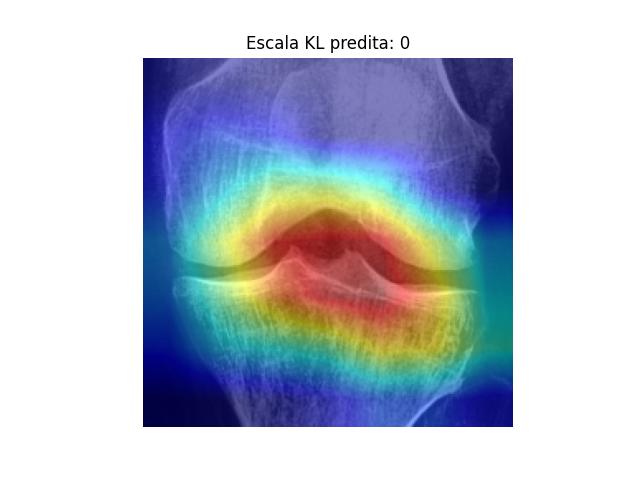
\includegraphics[width=0.15\textwidth]{figs/gradcams/gradcam_densenet169_kl0.png} & 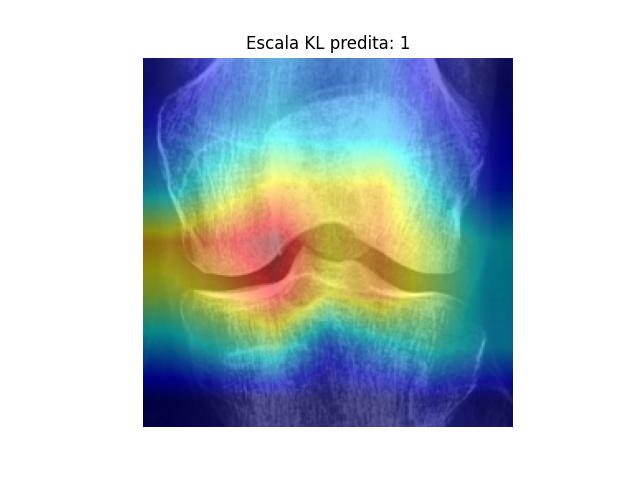
\includegraphics[width=0.15\textwidth]{figs/gradcams/gradcam_densenet169_kl1.png} & 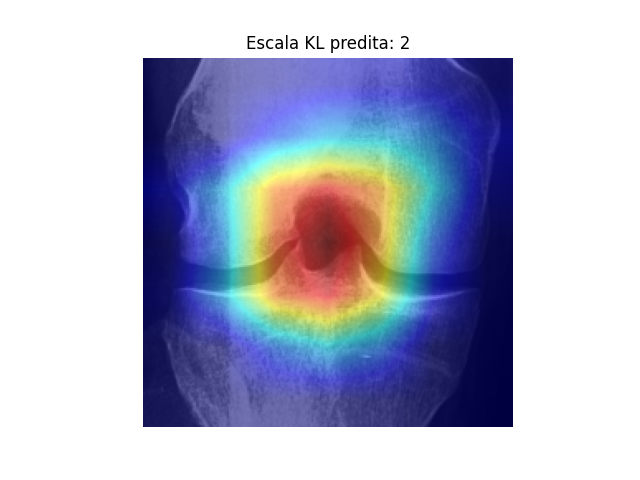
\includegraphics[width=0.15\textwidth]{figs/gradcams/gradcam_densenet169_kl2.png} & 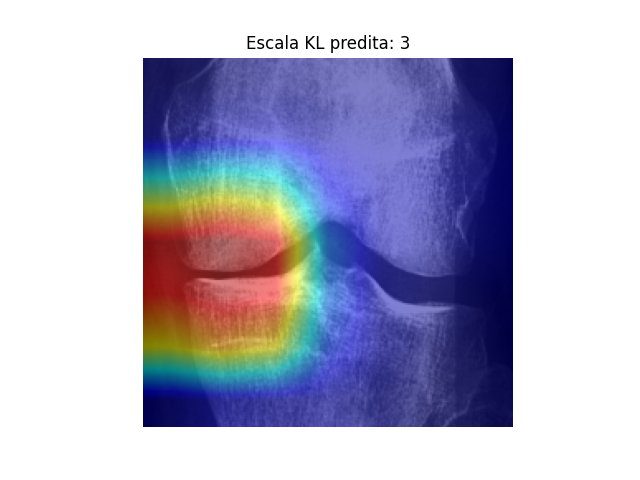
\includegraphics[width=0.15\textwidth]{figs/gradcams/gradcam_densenet169_kl3.png} & 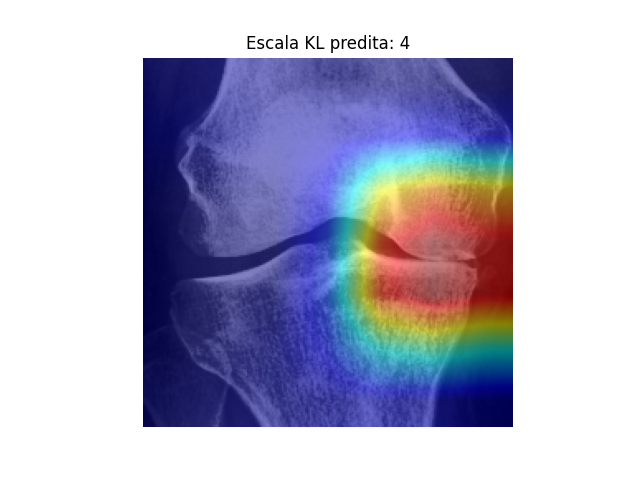
\includegraphics[width=0.15\textwidth]{figs/gradcams/gradcam_densenet169_kl4.png} \\ \hline
        DenseNet-121 & 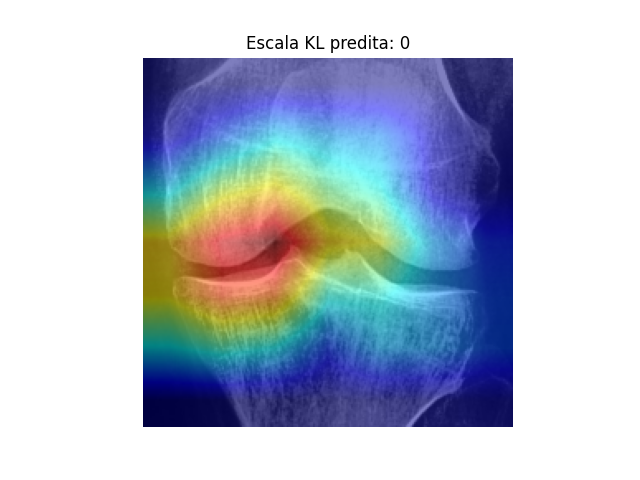
\includegraphics[width=0.15\textwidth]{figs/gradcams/gradcam_densenet121_kl0.png} & 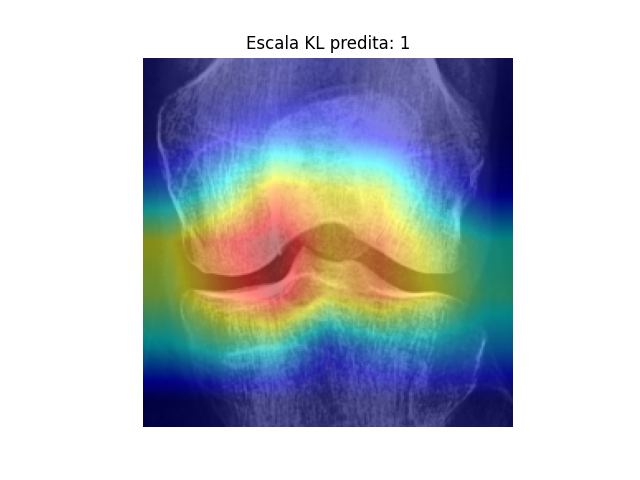
\includegraphics[width=0.15\textwidth]{figs/gradcams/gradcam_densenet121_kl1.png} & 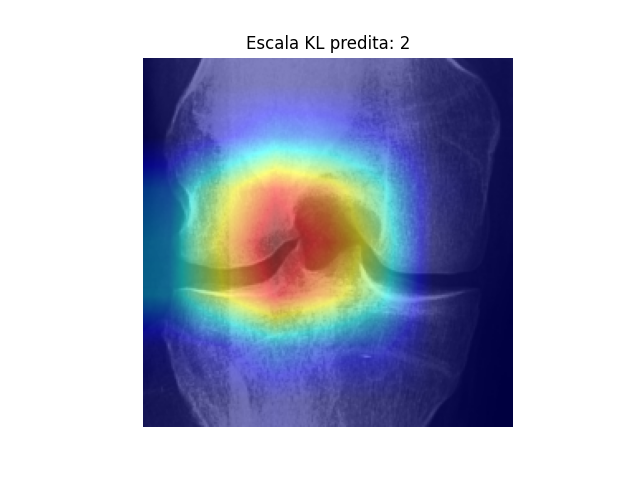
\includegraphics[width=0.15\textwidth]{figs/gradcams/gradcam_densenet121_kl2.png} & 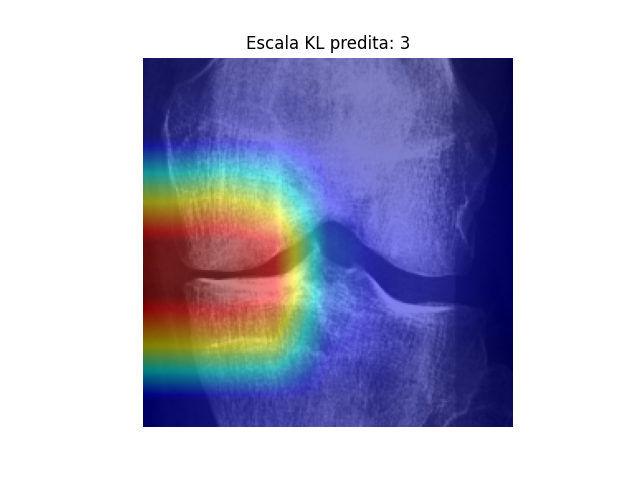
\includegraphics[width=0.15\textwidth]{figs/gradcams/gradcam_densenet121_kl3.png} & 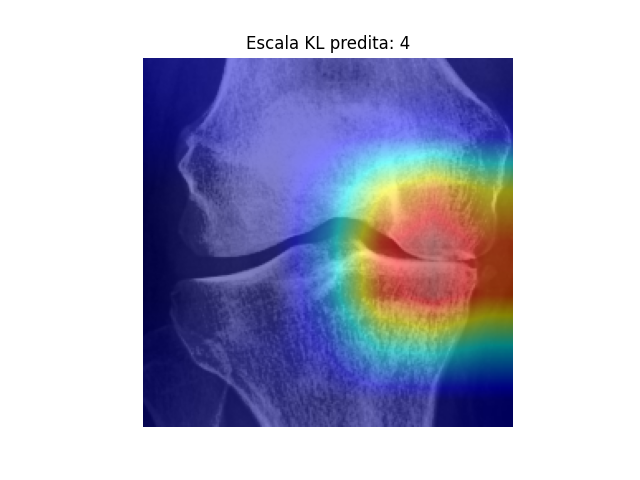
\includegraphics[width=0.15\textwidth]{figs/gradcams/gradcam_densenet121_kl4.png} \\ \hline
        GCViT-B & 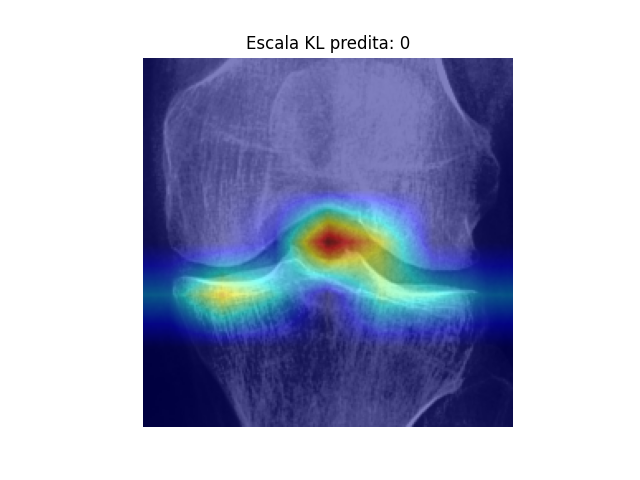
\includegraphics[width=0.15\textwidth]{figs/gradcams/gradcam_gcvit_kl0.png} & 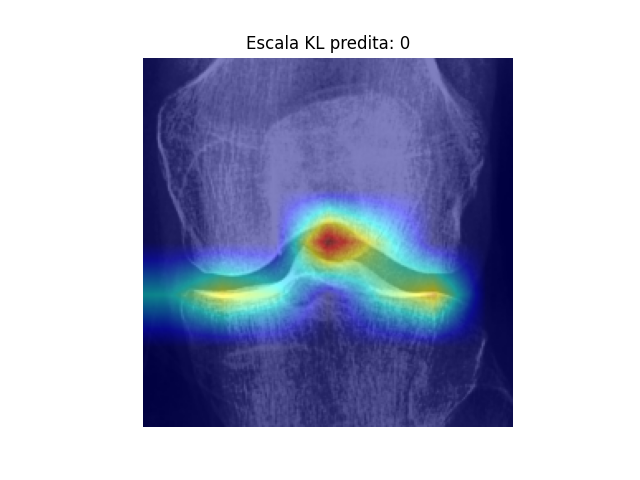
\includegraphics[width=0.15\textwidth]{figs/gradcams/gradcam_gcvit_kl1.png} & 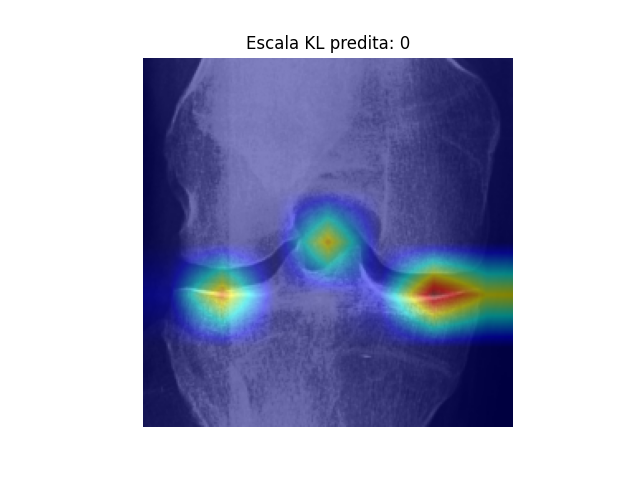
\includegraphics[width=0.15\textwidth]{figs/gradcams/gradcam_gcvit_kl2.png} & 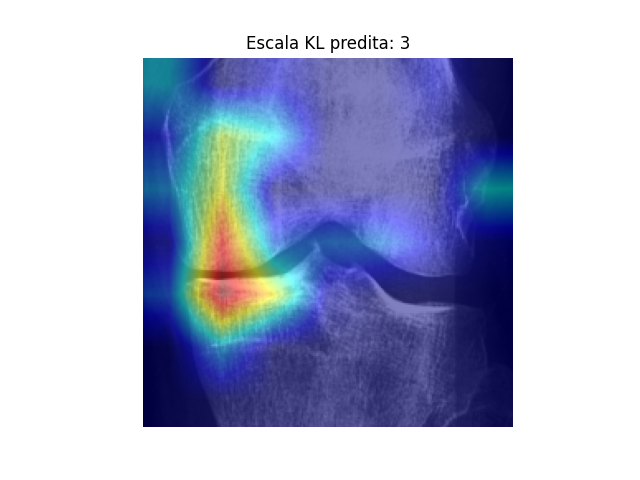
\includegraphics[width=0.15\textwidth]{figs/gradcams/gradcam_gcvit_kl3.png} & 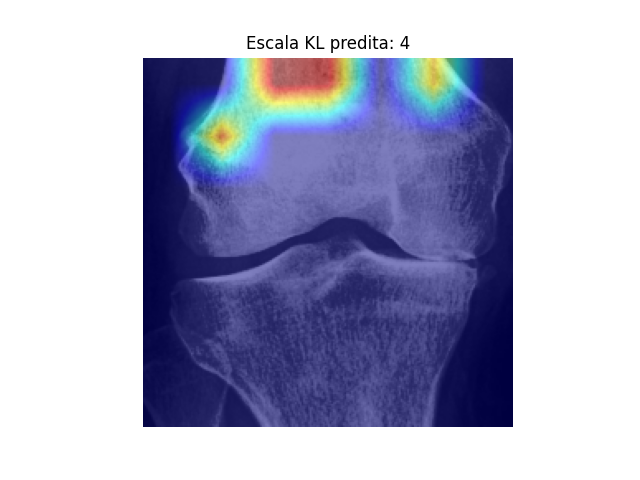
\includegraphics[width=0.15\textwidth]{figs/gradcams/gradcam_gcvit_kl4.png} \\ \hline
        DaViT-B & 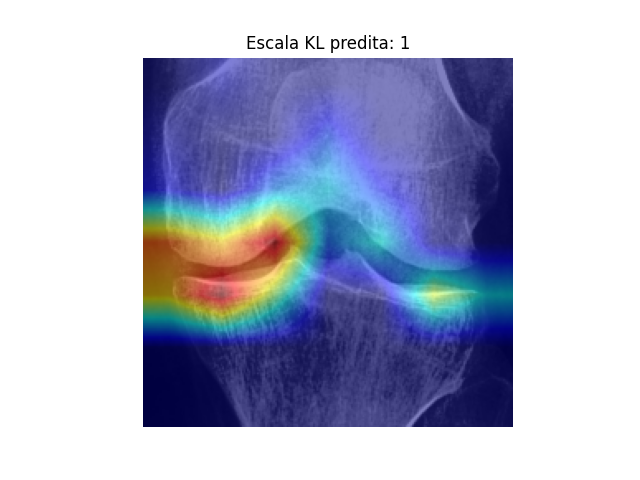
\includegraphics[width=0.15\textwidth]{figs/gradcams/gradcam_davit_kl0.png} & 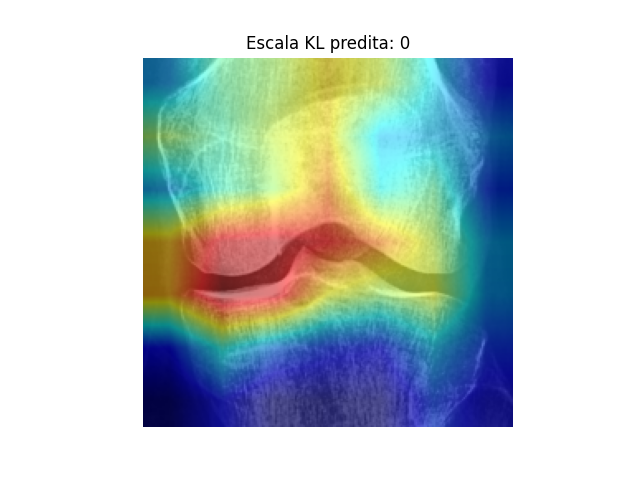
\includegraphics[width=0.15\textwidth]{figs/gradcams/gradcam_davit_kl1.png} & 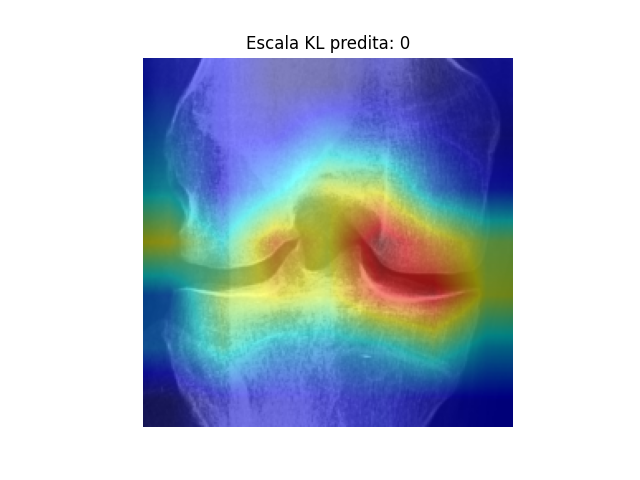
\includegraphics[width=0.15\textwidth]{figs/gradcams/gradcam_davit_kl2.png} & 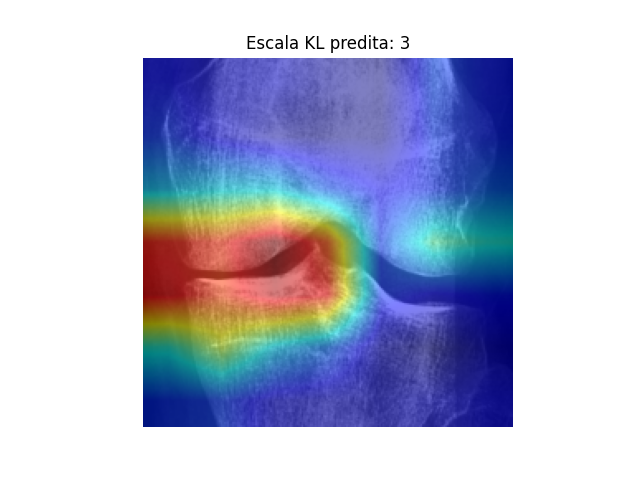
\includegraphics[width=0.15\textwidth]{figs/gradcams/gradcam_davit_kl3.png} & 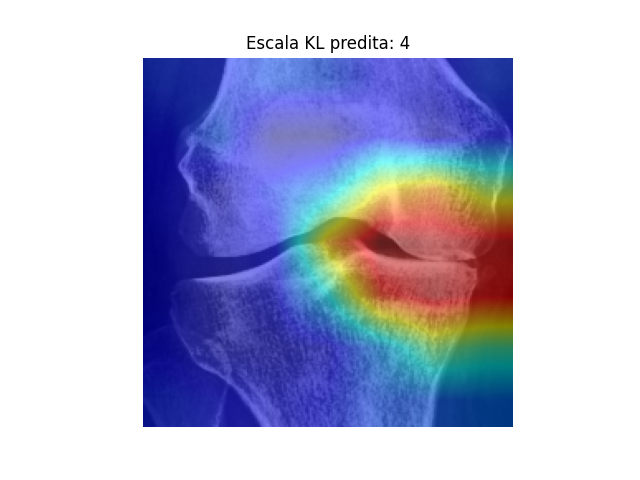
\includegraphics[width=0.15\textwidth]{figs/gradcams/gradcam_davit_kl4.png} \\ \hline
        MaxViT-T & 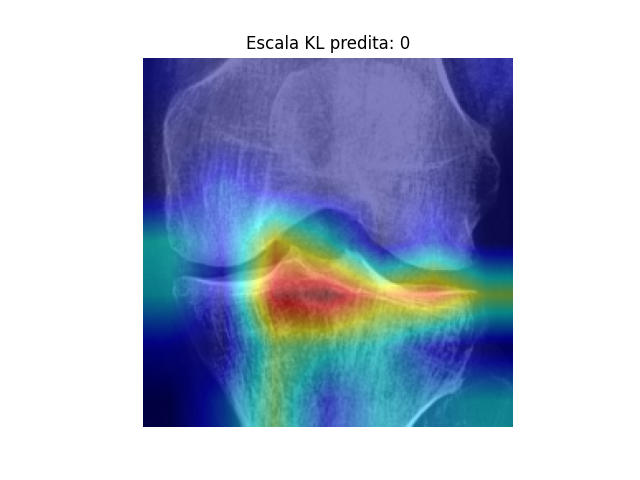
\includegraphics[width=0.15\textwidth]{figs/gradcams/gradcam_maxvit_kl0.png} & 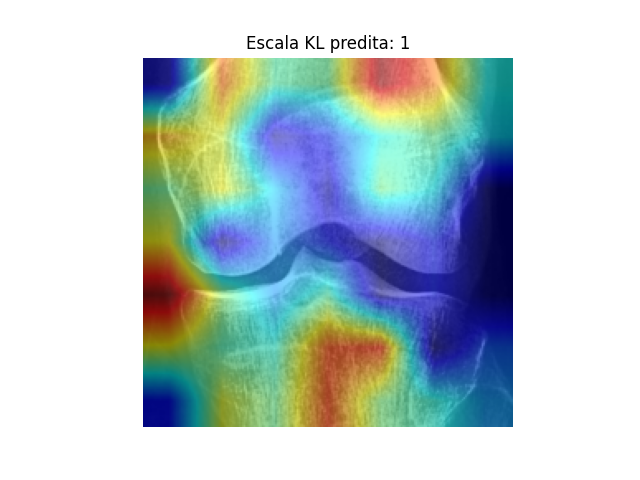
\includegraphics[width=0.15\textwidth]{figs/gradcams/gradcam_maxvit_kl1.png} & 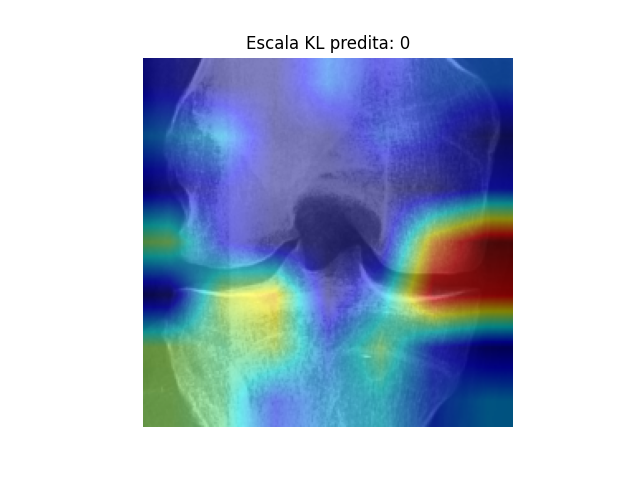
\includegraphics[width=0.15\textwidth]{figs/gradcams/gradcam_maxvit_kl2.png} & 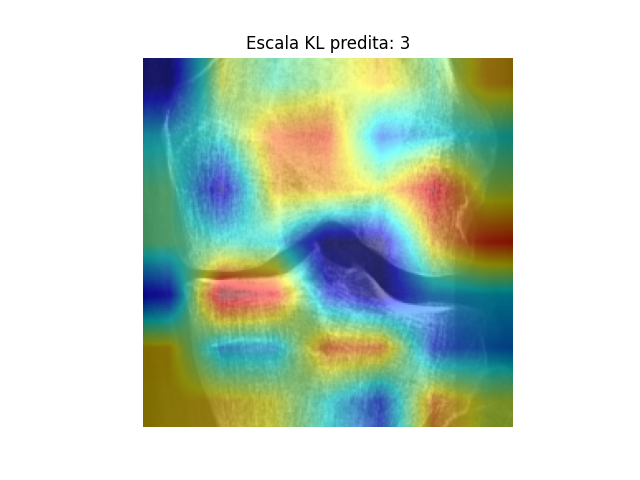
\includegraphics[width=0.15\textwidth]{figs/gradcams/gradcam_maxvit_kl3.png} & 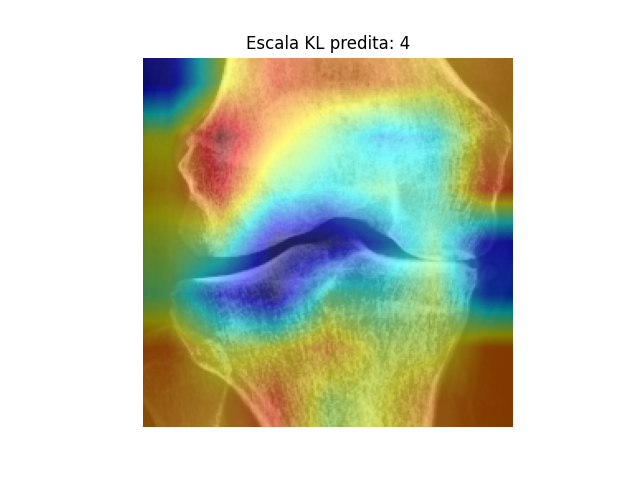
\includegraphics[width=0.15\textwidth]{figs/gradcams/gradcam_maxvit_kl4.png} \\ \hline
    \end{tabular}
    \caption{Visualização Grad-CAM para os melhores 5 modelos.}
    \label{tab:gradcams_top5_models}
\end{sidewaystable}

% De modo geral, os resultados indicam que os modelos de RNCs superaram os modelos de ViT, especialmente em termos de acurácia. Modelos como DenseNet-169, DenseNet-121 e Inception-v3 se destacaram, com acurácias gerais de 78.87\%, 77.09\% e 75.33\%, respectivamente. Os modelos de ViT, como DaViT-B e GCViT-B, também apresentaram resultados competitivos, com acurácias de 77.09\% e 75.55\%. No entanto, a performance de QWK foi muito próxima entre os modelos, indicando que ambas as arquiteturas são capazes de entender a natureza ordinal da classificação da OA de joelho e evitar erros significativos.

% Quanto à acurácia geral (\textit{overall}), todos os modelos apresentaram resultados razoavelmente bons, com valores variando de 0.6723 a 0.7319. Isso indica que todos os modelos foram capazes de aprender padrões relevantes para a classificação da OA de joelho. No entanto, é importante notar que o modelo DenseNet-169 obteve a maior acurácia geral, com um valor de 0.7319. Isso sugere que arquiteturas de RNCs densamente conectadas podem ser muito eficazes na extração de características relevantes em imagens médicas como radiografias de joelho. Além disso, os modelos de conexões residuais (ResNet) também apresentaram resultados competitivos, com acurácias gerais variando de 0.7044 a 0.7248, onde o ResNet-50 obteve a maior acurácia dentre eles e com o menor tempo de treinamento, oferecendo um bom equilíbrio entre generalização do modelo e custo computacional.

% Por outro lado, os modelos da família VGG (VGG-16 e VGG-19) apresentaram acurácias gerais mais baixas, variando de 0.6723 a 0.6851, o que sugere que essas arquiteturas mais simples podem não ser tão eficazes na extração de características complexas em radiografias de joelho. Embora fosse esperado que esses modelos tivessem desempenho inferior em relação aos modelos ResNet, devido à sua profundidade, os resultados indicam que esses modelos são capazes de aprender padrões relevantes e ter uma menor probabilidade de \textit{overfitting}, como observado no tempo de treinamento do VGG-16, que foi maior que a maioria dos modelos justamente por não ter parada antecipada em virtude da queda do erro no conjunto de validação.

% O GoogLeNet, com sua arquitetura Inception (versão 3), permitiu que o modelo tivesse uma acurácia geral de 0.7215, indicando que o modelo pode ser eficaz na extração de características relevantes e superar a maioria dos modelos de RNCs. Esse comportamento pode ser justificado pelo uso de uma técnica chamada de "bottleneck" ou "redução de dimensionalidade", que reduz a quantidade de parâmetros e a complexidade computacional do modelo, sem comprometer significativamente o desempenho.

% Os modelos de transformers, por sua vez, apresentaram acurácias gerais variando de 0.6862 a 0.7215, indicando que essas arquiteturas podem ser eficazes, mas talvez não sejam tão eficientes quanto os modelos de RNCs. O modelo Swin Transformer obteve a maior acurácia geral entre os modelos de transformers, com um valor de 0.6977, sugerindo que a abordagem hierárquica de atenção pode ser eficaz na extração de características relevantes em radiografias de joelho.

% Entretanto, é importante notar que a acurácia para a classe KL 1 foi baixa para todos os modelos, variando de 0.2562 e 0.4475. Isso indica que a classificação da OA de joelho no estágio 1 (duvidoso) pode ser mais desafiadora, possivelmente devido à semelhança visual com as classes adjacentes KL 0 e KL 2. Esse resultado pode ser observado na \autoref{confusion-matrix-resnet50}, que mostra a matriz de confusão do modelo ResNet-50. A classe KL 1 tem a menor acurácia dentre todas as classes, o que reflete o desafio na classificação dessa classe devido ao nível de detalhe ou até mesmo incoerência no rotulação das imagens do dataset.

% \begin{figure}
%     \centering
%     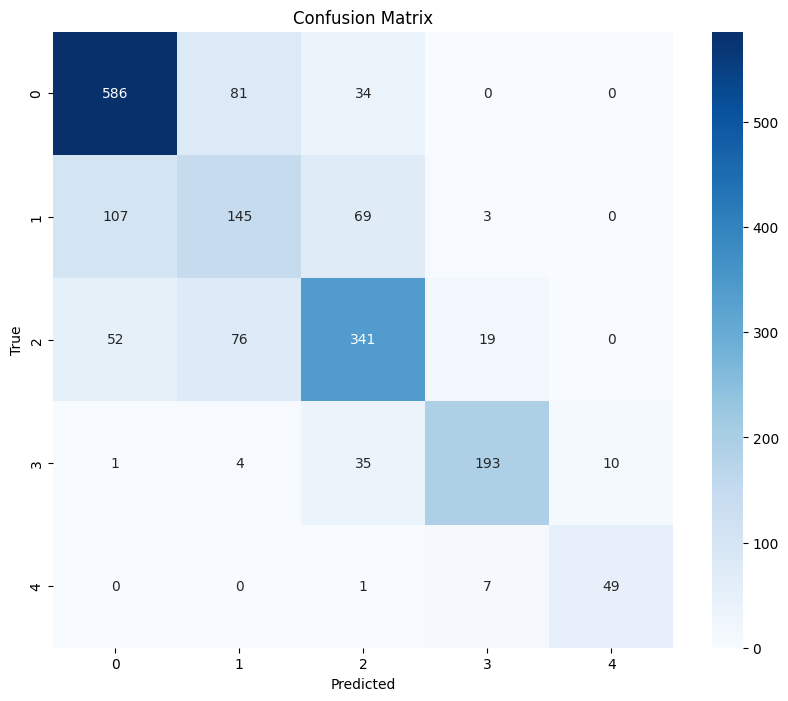
\includegraphics[width=\linewidth]{figs/confusion-matrix-resnet50.png}
%     \caption{Matriz de confusão do modelo ResNet-50.}
%     \label{confusion-matrix-resnet50}
% \end{figure}

% Em resumo, os modelos ResNet-50 e DenseNet-169 se destacaram em termos de tempo de treinamento e acurácia geral, respectivamente. No entanto, é importante considerar as características de cada classe ao escolher um modelo, pois diferentes modelos podem ter desempenhos diferentes para cada classe.

% A \autoref{tab:resultados-corn} apresenta os resultados dos modelos de RNCs e ViTs treinados para a classificação da OA de joelho usando a função de perda CORN. Em relação ao tempo de treinamento, não houve uma mudança significativa comparado com a função de perda \textit{crossentropy}. O modelo mais rápido foi, novamente, o ResNet-50, com um tempo de 10.32 segundos, enquanto o modelo mais lento foi o Swin Transformer, com um tempo de 35.58 segundos. Em relação à acurácia geral, os resultados variaram de 0.6546 a 0.7181, indicando que a função de perda CORN pode ser eficaz na classificação da OA de joelho, mas não necessariamente supera a função de perda \textit{crossentropy}. Isso é justificado pelo fato de que a função de perda CORN é mais adequada quando o modelo faz predições mais afastadas do rótulo real, o que não foi evidenciado ao observar as matrizes de confusão dos modelos.

% \begin{table}
%     \centering
%     \begin{tabular}{|c|c|c|c|c|c|c|c|}
%         \hline
%         \multirow{2}{*}{Modelo} & \multirow{2}{*}{Tempo} & \multirow{2}{*}{Overall} & \multicolumn{5}{|c|}{Classe KL} \\ \cline{4-8}
%         &  &  & 0 & 1 & 2 & 3 & 4 \\ \hline
%         ResNet-34 & 14.93 & 0.6895 & 0.7518 & 0.5586 & 0.6107 & 0.8107 & 0.8246 \\ \hline
%         ResNet-50 & 10.32 & 0.7181 & 0.796 & 0.5031 & 0.6824 & 0.823 & 0.8421 \\ \hline
%         ResNet-101 & 16.17 & 0.6994 & 0.7418 & 0.4506 & 0.707 & 0.8519 & 0.8772 \\ \hline
%         VGG-16 & 19.29 & 0.6762 & 0.7646 & 0.358 & 0.6824 & 0.7984 & 0.8246 \\ \hline
%         VGG-19 & 24.05 & 0.6669 & 0.7974 & 0.3549 & 0.6066 & 0.7901 & 0.8246 \\ \hline
%         DenseNet-121 & 10.62 & 0.6911 & 0.729 & 0.4444 & 0.7172 & 0.8272 & 0.8246 \\ \hline
%         DenseNet-169 & 13.75 & 0.717 & 0.7874 & 0.5833 & 0.6393 & 0.8148 & 0.8596 \\ \hline
%         Inception-v3 & 17.09 & 0.701 & 0.7932 & 0.5093 & 0.6639 & 0.7325 & 0.8421 \\ \hline
%         ViT-B & 36.97 & 0.6817 & 0.7447 & 0.4815 & 0.6393 & 0.8066 & 0.8772 \\ \hline
%         DeiT & 34.73 & 0.6602 & 0.7047 & 0.4877 & 0.6209 & 0.7984 & 0.8421 \\ \hline
%         Swin & 35.58 & 0.6546 & 0.7803 & 0.4658 & 0.6722 & 0.8395 & 0.7894 \\ \hline
%     \end{tabular}
%     \caption{Desempenho dos modelos de RNCs e ViTs na classificação da OA de joelho usando a função da perda CORN.}
%     \label{tab:resultados-corn}
%     \end{table}

% No entanto, é importante notar que o modelo ResNet-50 obteve a maior acurácia geral, com um valor de 0.7181, superando os demais modelos, inclusive o modelo DenseNet-169, que obteve a maior acurácia geral com a função de perda \textit{crossentropy}. Isso sugere que a função de perda CORN pode ser eficaz em arquiteturas de RNCs, especialmente aquelas com conexões residuais. Entretanto, o modelo DenseNet-169 foi quem obteve a maior acurácia para a classe KL 1, com um valor de 0.5833, que é a classe mais desafiadora de ser classificada, como observado anteriormente.

% \section{Resultados e Discussão}

% \subsection{Visão Geral dos Resultados}

% Os experimentos envolveram avaliação de 18 arquiteturas (CNN e ViT), cada uma treinada com duas funções de perda: \emph{cross entropy} e \emph{Corn} (cumulative ordinal regression). As métricas principais consideradas foram acurácia, kappa de Cohen (coeficiente de concordância), weighted Quadratic Weighted Kappa (QWK) e Mean Absolute Error (MAE). A Tabela~\ref{tab:resultados} resume os cinco modelos com melhor desempenho em termos de QWK, para ambas as funções de perda.

% \subsection{Discussão}

% Observa-se que o modelo \textbf{GCViT} apresentou o melhor desempenho global, atingindo QWK de 0.8725 com \emph{cross entropy} e 0.8752 com \emph{Corn}, além de MAE mínimo de 0.29399 e 0.29123, respectivamente;:contentReference[oaicite:1]{index=1}. Logo em seguida, os modelos \textbf{DaViT} e \textbf{MaxViT\_T} também se destacaram, com QWK acima de 0.86 e MAE abaixo de 0.32, evidenciando a eficácia de transformers especializados para tarefas de classificação ordinal de osteoartrite.

% Entre as CNNs, as versões densas (\emph{DenseNet169} e \emph{DenseNet121}) obtiveram desempenhos notáveis, com QWK acima de 0.85 e acurácias próximas a 72\% sob \emph{cross entropy}, mas ficaram abaixo dos ViTs em QWK e MAE;:contentReference[oaicite:3]{index=3}.

% Ainda, a função de perda \emph{Corn} mostrou ligeira melhora em QWK para a maioria dos modelos de ViT, embora com tempo de treinamento tipicamente maior do que com \emph{cross entropy} (por exemplo, GCViT: 3454\,s vs.\ 2423\,s);:contentReference[oaicite:5]{index=5}.

% \begin{table}[htb]
% \centering
% \caption{Desempenho dos cinco melhores modelos (ordem por QWK) para as duas funções de perda.}
% \label{tab:resultados}
% \begin{tabular}{l|ccccc|ccccc}
% \hline
% \multirow{2}{*}{\textbf{Modelo}} & \multicolumn{5}{c|}{\textbf{Cross Entropy}} & \multicolumn{5}{c}{\textbf{Corn}} \\
%  & Acc. & Kappa & QWK & MAE & Tempo (s) & Acc. & Kappa & QWK & MAE & Tempo (s) \\
% \hline
% GCViT        & 0.7363 & 0.6372 & 0.8725 & 0.29399 & 3454.0 & 0.7347 & 0.6369 & 0.8752 & 0.29123 & 2422.6 \\
% DaViT        & 0.7358 & 0.6362 & 0.8647 & 0.30226 & 3045.0 & 0.7286 & 0.6288 & 0.8713 & 0.29950 & 2342.1 \\
% MaxViT\_T    & 0.7220 & 0.6165 & 0.8616 & 0.31550 & 1489.6 & 0.7038 & 0.5934 & 0.8636 & 0.32267 & 1006.4 \\
% DenseNet169  & 0.7220 & 0.6158 & 0.8519 & 0.32488 &  888.2 & 0.7187 & 0.6143 & 0.8660 & 0.31219 & 1345.6 \\
% DenseNet121  & 0.7204 & 0.6110 & 0.8514 & 0.32708 & 1148.4 & 0.7071 & 0.6001 & 0.8592 & 0.32377 &  624.8 \\
% \hline
% \end{tabular}
% \end{table}

% \subsection{Principais Conclusões}

% \begin{itemize}
%   \item \textbf{GCViT} foi o modelo de melhor desempenho, com QWK máximo de 0.8752 e MAE mínimo de 0.2912, indicando superior capacidade de modelar a natureza ordinal da escala KL.
%   \item Transformers (GCViT, DaViT, MaxViT\_T) superaram consistentemente as CNNs clássicas em QWK e MAE, embora demandem maior custo computacional.
%   \item A função de perda \emph{Corn} proporcionou ganhos moderados em QWK para ViTs, justificando seu uso em tarefas de classificação ordinal.
%   \item Dentre as CNNs, \emph{DenseNet169} e \emph{DenseNet121} foram as mais competitivas, alcançando QWK acima de 0.85.
% \end{itemize}
